\documentclass{ltjarticle}

\usepackage{graphicx}

\usepackage[backend=biber,style=numeric]{biblatex}
\addbibresource{references.bib}

\title{Identifying Woodblocks from the Bukan Collection}
\author{Thomas Leyh}
\date{March 20th, 2020}

\begin{document}

\maketitle

\section{Introduction}

The \emph{Center for Open Data in the Humanities} (CODH) is a joint research institution in Tokyo, Japan. Its goal is the promotion of data-driven research in the humanities.\cite{kitamoto2017codh} For this purpose they were releasing a number of data sets, all of them related to Japanese history and arts. This work started out by specifically looking at the \emph{Bukan Collection}\cite{codh2018bukan}, around 370 books with information about government officials during the 18th and 19th century. So, how can we assist humanities researchers with techniques from Computer Science?

By applying well-known algorithms from Computer Vision on the books' pages, without using information about the written content, we were able to develop a reliable system for spotting and visualizing similarities. This might be a first step into building a timeline of a book's prints, thus exposing some historical events hidden in there.

But more importantly, this is an example of how even conservative algorithms can give compelling results by using a few reasonable assumptions on the corresponding data. Even basic computer-aided quantitative analysis might reveal information that is near invisible of a human researcher.

\subsection{The Bukan Collection}

This work was mainly concerned with extracting information from a specific type of book: 武鑑---Bukan. These are historic Japanese books from Edo period (1603-1868). They are about listing people of influence, i.e. persons, families and institutions with governmental responsibilities. Alongside names, there are also various symbols like family crests and procession items as well as family trees. The books are written in pre-modern Japanese (\emph{Kuzushiji}), therefore they can not easily be read without special training. See figure~\ref{fig:shuugyokubukan006} for an example.

\begin{figure}[]
    \centering
    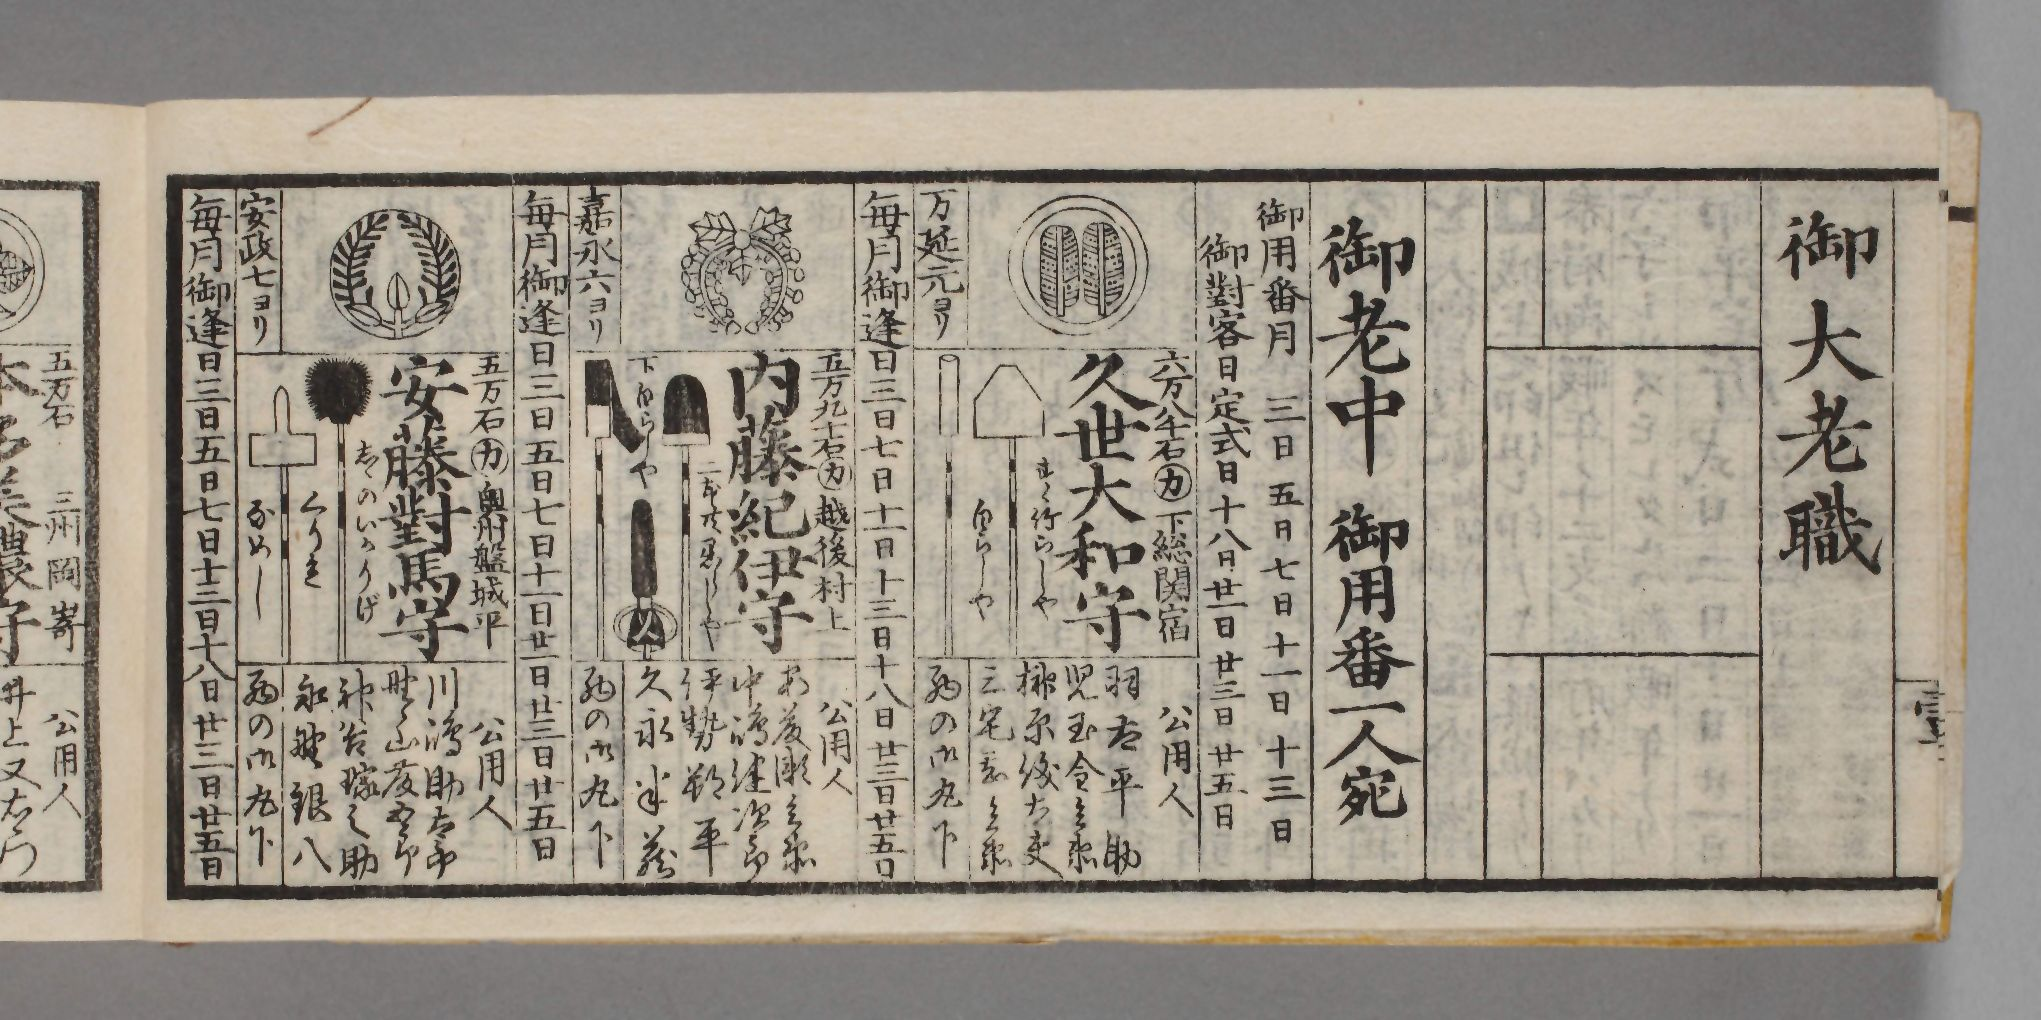
\includegraphics[width=\textwidth]{200019500_00006.jpg}
    \caption[Shūgyoku Bukan (袖玉武鑑), page 6]{Shūgyoku Bukan (袖玉武鑑) from 1861, page 6; showing names, descriptions, family crests and procession items. Especially interesting are the blank areas on the right. These might be filled in later prints.}
    \label{fig:shuugyokubukan006}
\end{figure}

Back then, the Bukan were bestsellers. Often, it was vital knowledge to be able to identify feudal lords and their subordinates. Mistakes when determining the difference in status could easily lead to dispute, sometimes even in a violent manner.\cite{dower1990elements} Nevertheless, publishing of the Bukan was not centralized and therefore not standardized. Especially the layout of the pages---even of books from the same year---might differ to some degree.

The language barrier and the layout difference might seem to complicate the application of common algorithms from Natural Language Processing and Computer Vision. But utilizing the knowledge about the specific data at hand, about the Bukan and especially about their production, we define a problem that is more approachable. This can be done by looking at the printing process.

The books were created using Japanese woodblock-printing. Specialized craftspeople were carving out whole pages from wood. By applying ink on these blocks, numerous prints could be created with comparatively low costs per unit. But it is not like all pages made with the same woodblock would look identical. On the one hand, there are differences in quality of the printed page, stemming from e.g. the amount of ink or the state of the woodblock. On the other hand, the woodblocks itself might have been modified between prints. Some names could have been added, some removed or some symbols modified.

These differences can indicate historical occurrences. Changing family structures like births and deaths as well as gain or loss of status. A scholar in history and old literature will be able to interpret these findings. This work is about supplying her with interactive tools for quickly spotting such sections of interest.

\section{Method}

For tackling this task, three common techniques are used:

\begin{enumerate}
    \item \emph{Keypoint Detection and Matching}, a method from Computer Vision used for finding the same object in different images.
    \item \emph{Projective Transformation} for comparing two different images, regardless their original orientation.
    \item \emph{Relational Databases} for easily storing results as well as querying for relevant pages.
\end{enumerate}

At the end there will be a database populated with the necessary data for easily browsing books, finding similar pages and quickly displaying visualizations. For all these steps free and open tools are available. Especially for the Computer Vision parts the mature \emph{OpenCV} software library was used.\cite{opencv_library}

\subsection{Keypoint Matching}

\subsection{Projective Transformation}

\subsection{Relational Databases}

\printbibliography

\end{document}
